\normaltrue
\correctionfalse

%\UPSTIidClasse{11} % 11 sup, 12 spé
%\newcommand{\UPSTIidClasse}{12}

\exer{Fixation de ski de randonnée $\star$ \label{A5:05:76}}
\setcounter{question}{0}
%\UPSTIcompetence[2]{A5-05}
%\UPSTIcompetence[2]{A5-04}

\index{Compétence A5-05}
\index{Compétence A5-04}

\index{GPS}
\index{Spécification géométrique des produits}
\index{Roue motrice}

\ifcorrection
\else
\marginnote{\textbf{Pas de corrigé pour cet exercice.}}
\fi

\ifprof
\else


On considère le platine d'une fixation de ski de randonnée.

\begin{center}
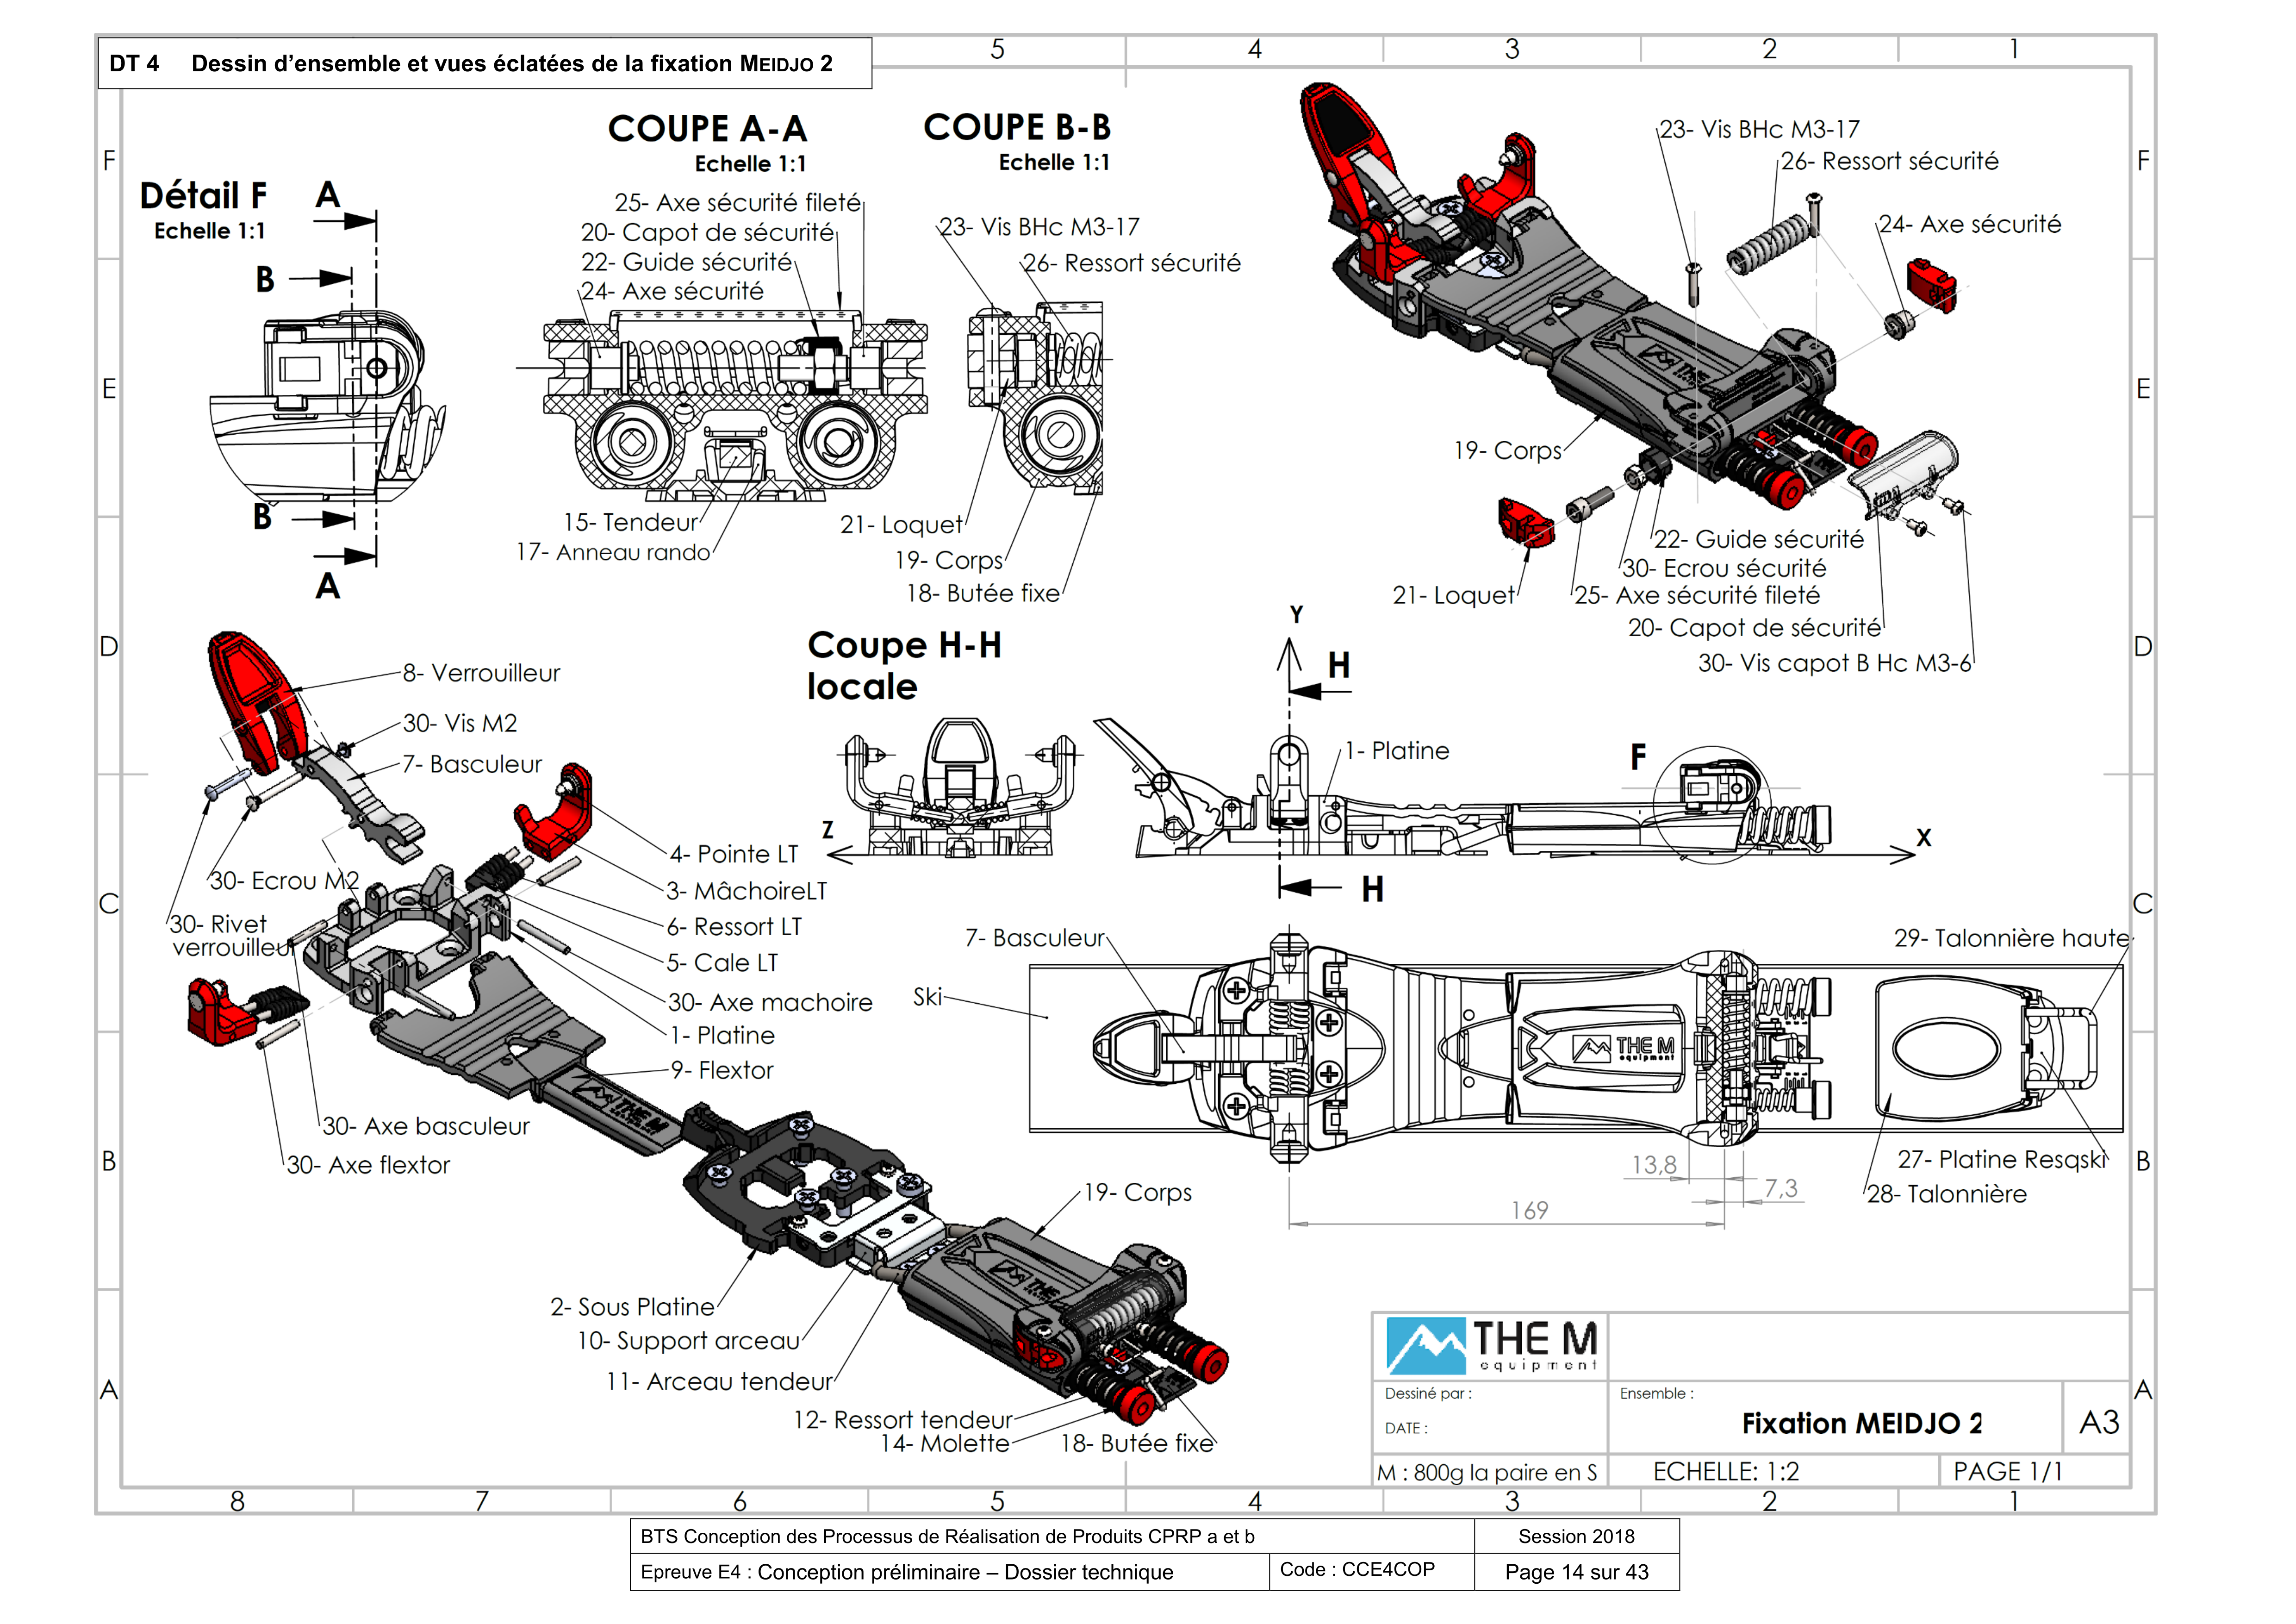
\includegraphics[width=\linewidth]{76_01}
\end{center}



\fi



\question{Justifier pourquoi les surfaces A, B et C ont été choisies comme éléments de référence ?}
\ifprof
\else
\fi


\question{Décoder les spécifications suivantes : \includegraphics[height=2cm]{76_04}. Pour la spécification d'enveloppe, tracer le gabarit associé.}
\ifprof
\else
\fi

\question{Décoder la spécification suivante \includegraphics[height=0.8cm]{76_05}.}
\ifprof
\else
\fi

\question{Ajouter une spécification de planéité avec une tolérance $t_p$ sur le plan A.}
\ifprof
\else
\fi

\question{Ajouter une spécification de perpendicularité $t_p$ avec une tolérance $t_p$ entre A et B. Décoder la spécification.}
\ifprof
\else
\fi

\begin{figure*}[!h]
\includegraphics[width=\linewidth]{76_03.png}
\end{figure*}

\ifprof
\else
\begin{flushright}
\footnotesize{Corrigé  voir \ref{A5:05:76}.}
\end{flushright}%
\fi 